\documentclass[12pt]{article}
\usepackage[utf8]{inputenc}
\usepackage[spanish]{babel}
\usepackage{amsmath}
\usepackage[a4paper, total={7in, 10in}]{geometry}
\usepackage{listings}
\usepackage{xcolor}
\usepackage{lipsum}
\usepackage{graphicx}
\usepackage{subcaption}
\usepackage{biblatex}
\addbibresource{referencias.bib}
\definecolor{codegreen}{rgb}{0,0.6,0}
\definecolor{codegray}{rgb}{0.5,0.5,0.5}
\definecolor{codepurple}{rgb}{0.58,0,0.82}
\definecolor{backcolour}{rgb}{0.95,0.95,0.92}

\lstdefinestyle{mystyle}{
	backgroundcolor=\color{backcolour},   
	commentstyle=\color{codegreen},
	keywordstyle=\color{magenta},
	numberstyle=\tiny\color{codegray},
	stringstyle=\color{codepurple},
	basicstyle=\ttfamily\footnotesize,
	breakatwhitespace=false,         
	breaklines=true,                 
	captionpos=b,                    
	keepspaces=true,                 
	numbers=left,                    
	numbersep=5pt,                  
	showspaces=false,                
	showstringspaces=false,
	showtabs=false,                  
	tabsize=2
}
\lstset{style=mystyle}

\title{Proyecto del curso CC112}
\author{Edwin Arles Requena Alvarado, Walter Arath Bill Iizarbe Marchan, Zósimo Clemente Barrientos Huamaní}

\begin{document}
	%Alternativa de título
	\begin{center}
		\textbf{\huge Proyecto del Curso CC112}
	\end{center}
	\vspace{1cm}
	%Alternativa de autores
	\noindent
	\begin{tabular*}{\textwidth}{@{\extracolsep{\fill}} c c c @{}}
\begin{tabular}{@{}c@{}}
	{\footnotesize \textbf{Edwin Arles Requena Alvarado}} \\
	{\footnotesize \textit{Escuela de Ciencia de la computación}} \\
	{\footnotesize \textit{Universidad Nacional de Ingeniería}} \\
	{\footnotesize Lima, Perú} \\
	{\footnotesize \texttt{edwin.requena.a@uni.pe}}
\end{tabular} &
\begin{tabular}{@{}c@{}}
	{\footnotesize \textbf{Walter Arath Bill Iizarbe Marchan}} \\
	{\footnotesize \textit{Escuela de Física}} \\
	{\footnotesize \textit{Universidad Nacional de Ingeniería}} \\
	{\footnotesize Lima, Perú} \\
	{\footnotesize \texttt{walter.iilizarbe.m@uni.pe}}
\end{tabular} &
\begin{tabular}{@{}c@{}}
	{\footnotesize \textbf{Zósimo C. Barrientos Huamaní}} \\
	{\footnotesize \textit{Escuela de Ingeniería Física}} \\
	{\footnotesize \textit{Universidad Nacional de Ingeniería}} \\
	{\footnotesize Lima, Perú} \\
	{\footnotesize \texttt{zosimo.barrientos.h@uni.pe}}
\end{tabular}

	\end{tabular*}
	
	\section{Introduccion}
	El presente proyecto tiene como objetivo principal proporcionar a los estudiantes una introducción práctica al lenguaje Python. Este proyecto está diseñado para que los alumnos puedan aplicar los conceptos aprendidos en C++ en un entorno diferente, comprender las ventajas de Python en términos de sintaxis, productividad y su aplicabilidad en diversas áreas tecnológicas. 
	
	Además, se espera que los estudiantes experimenten con aplicaciones reales que utilizan Python, motivándolos a explorar más sobre inteligencia artificial, desarrollo web y ciencia de datos. Este proyecto también busca ampliar sus habilidades de programación y sus perspectivas sobre el uso práctico de diferentes lenguajes de programación en el mundo real.
	
	A lo largo del proyecto, se destacarán las diferencias y similitudes entre C++ y Python, dos lenguajes de programación orientados a objetos ampliamente utilizados en la industria. Mientras que C++ es conocido por su eficiencia en el desarrollo de sistemas operativos, aplicaciones, navegadores y juegos, Python se destaca por su versatilidad y su amplia adopción en ciencia de datos, aprendizaje automático, desarrollo web y muchas otras áreas tecnológicas.
	
	\section{Objetivos}
	El proyecto tiene como objetivo proporcionar a los estudiantes una introducción práctica al lenguaje Python, permitiéndoles:
	\begin{itemize}
		\item Aplicar los conceptos aprendidos en C++ en un entorno diferente.
		\item Comprender las ventajas de Python en términos de sintaxis, productividad y aplicabilidad en diversas áreas tecnológicas.
		\item Experimentar con aplicaciones reales que utilizan Python, motivándolos a explorar más sobre inteligencia artificial, desarrollo web y ciencia de datos.
		\item Ampliar sus habilidades de programación y perspectivas sobre el uso práctico de diferentes lenguajes de programación en el mundo real.
	\end{itemize}
	
	\section{Marco Teórico}
	
	\subsection{Características de Python}
	
	Python posee varias características distintivas:
	\begin{itemize}
		\item \textbf{Simplicidad y legibilidad}: La sintaxis de Python está diseñada para ser fácil de leer y escribir, lo que permite a los desarrolladores expresar conceptos en menos líneas de código.
		\item \textbf{Interactividad}: Python es un lenguaje interpretado, lo que permite a los desarrolladores probar fragmentos de código rápidamente.
		\item \textbf{Portabilidad}: Python es multiplataforma, es decir, puede ejecutarse en diversos sistemas operativos sin necesidad de modificaciones significativas en el código.
		\item \textbf{Amplia biblioteca estándar}: Python cuenta con una extensa biblioteca estándar que proporciona módulos y paquetes para prácticamente cualquier tarea.
		\item \textbf{Soporte para múltiples paradigmas}: Python soporta programación orientada a objetos, programación funcional y programación imperativa.
	\end{itemize}
	
	\subsection{Definición y Contexto de C++}
	
	C++ es un lenguaje de programación de propósito general, conocido por su eficiencia y flexibilidad. Fue desarrollado por Bjarne Stroustrup y apareció por primera vez en 1985 como una extensión del lenguaje C. De acuerdo con E Balaguruswamy en "Object Oriented Programming With C++" y Hari Mohan Pandey en "Object - Oriented Programming C++ Simplified", C++ es ampliamente utilizado en el desarrollo de sistemas operativos, software de alto rendimiento, aplicaciones en tiempo real y videojuegos.
	
	\subsubsection{Características de C++}
	
	C++ tiene varias características clave:
	\begin{itemize}
		\item \textbf{Eficiencia y rendimiento}: C++ permite un control preciso sobre los recursos del sistema, lo que lo hace ideal para aplicaciones de alto rendimiento.
		\item \textbf{Programación orientada a objetos (OOP)}: C++ soporta plenamente la OOP, facilitando la creación de aplicaciones modulares y reutilizables.
		\item \textbf{Compatibilidad con C}: C++ es compatible con el lenguaje C, lo que permite a los desarrolladores utilizar bibliotecas y código C existentes.
		\item \textbf{Flexibilidad}: C++ proporciona una gran cantidad de herramientas y características que permiten a los desarrolladores trabajar a un alto nivel de abstracción o a un nivel muy bajo cercano al hardware.
	\end{itemize}
	
	\subsection{Comparación entre Python y C++}
	
	\subsubsection{Sintaxis y Facilidad de Uso}
	
	Python es conocido por su sintaxis simple y legible, lo que facilita el aprendizaje y reduce el tiempo de desarrollo. Según Linge y Langtangen, Python permite a los desarrolladores centrarse en resolver problemas en lugar de preocuparse por detalles de sintaxis complejos. Por otro lado, C++ tiene una sintaxis más compleja y estricta, lo que puede aumentar la curva de aprendizaje, pero ofrece un control más detallado sobre el hardware y los recursos del sistema.
	
	\subsubsection{Productividad y Eficiencia}
	
	Python es ideal para desarrollo rápido y prototipado gracias a su sintaxis concisa y a la disponibilidad de bibliotecas para diversas tareas. Sin embargo, C++ es superior en términos de rendimiento y eficiencia, lo que lo hace más adecuado para aplicaciones que requieren un uso intensivo de recursos, como los videojuegos y sistemas en tiempo real.
	
	\subsubsection{Áreas de Aplicación}
	
	Python es ampliamente utilizado en ciencia de datos, inteligencia artificial, desarrollo web y automatización, debido a su simplicidad y a la disponibilidad de poderosas bibliotecas como Pandas, NumPy, TensorFlow y Django. En contraste, C++ es predominante en el desarrollo de sistemas operativos, motores de juegos, software embebido y aplicaciones de alta performance, donde el control de recursos y la eficiencia son críticos.
	
	\subsection{Aplicaciones Reales de Python}
	
	Según Linge y Langtangen, Python es una herramienta poderosa en ciencia de datos y análisis, facilitando el procesamiento y la visualización de grandes conjuntos de datos. En inteligencia artificial, Python es el lenguaje de elección debido a bibliotecas como TensorFlow y PyTorch, que permiten la creación y entrenamiento de modelos de aprendizaje profundo. En el desarrollo web, frameworks como Django y Flask simplifican la creación de aplicaciones web robustas y escalables.
	
	\subsection{Aplicaciones Reales de C++}
	
	De acuerdo con Balaguruswamy y Pandey, C++ se utiliza ampliamente en el desarrollo de sistemas operativos como Windows y Linux, así como en software de control en tiempo real. En la industria de los videojuegos, motores de juegos como Unreal Engine están escritos en C++, aprovechando su capacidad para manejar gráficos complejos y cálculos intensivos. Además, C++ es fundamental en sistemas embebidos y dispositivos IoT, donde la eficiencia y el control del hardware son esenciales.
	
	\subsection*{Conclusión del Marco Teórico}
	
	En resumen, tanto Python como C++ tienen sus fortalezas y aplicaciones específicas. Python sobresale en productividad, simplicidad y su uso en áreas emergentes como la inteligencia artificial y la ciencia de datos. Por otro lado, C++ ofrece un control y eficiencia incomparables, siendo crucial en aplicaciones de alto rendimiento y sistemas en tiempo real. Conocer ambos lenguajes proporciona a los estudiantes una visión amplia y versátil del desarrollo de software, preparándolos para enfrentar una variedad de desafíos tecnológicos en el mundo real.
	\vspace{0.2cm}
	
	\section{Desarrollo}
	El siguiente código de Python ilustra un proyecto básico de machine learning centrado en la regresión lineal utilizando el conjunto de datos de diabetes proporcionado por la biblioteca sklearn. A continuación se presenta una explicación detallada del código en varios párrafos.
	
	Primero, se importan las bibliotecas necesarias: numpy para operaciones numéricas, matplotlib.pyplot para la visualización de datos y sklearn para cargar el conjunto de datos y los modelos de regresión. Se utiliza el conjunto de datos de diabetes, que se carga con load\_diabetes(), proporcionando las características (data) y los valores objetivo (target). Estos datos se almacenan en las variables a y b respectivamente.
	
	\begin{lstlisting}[language=Python]
	import numpy as np
	import matplotlib.pyplot as plt
	from sklearn.datasets import load_diabetes
	from sklearn.linear_model import LinearRegression, Ridge, Lasso
	
	# Cargar el conjunto de datos de diabetes
	diabetes = load_diabetes()
	a = diabetes.data
	b = diabetes.target
	\end{lstlisting}
	
	A continuación, se definen tres modelos de regresión diferentes: regresión lineal, regresión Ridge y regresión Lasso. Estos modelos se inicializan con sus respectivos hiperparámetros, donde alpha es un parámetro de regularización para Ridge y Lasso. La regresión lineal se define sin parámetros adicionales, mientras que Ridge se inicializa con alpha=1.0 y Lasso con alpha=0.1.
	
	\begin{lstlisting}[language=Python] 
	import matplotlib.pyplot as plt
	from sklearn.datasets import load_diabetes
	from sklearn.linear_model import LinearRegression, Ridge, Lasso
	# Cargar el conjunto de datos de diabetes
	diabetes = load_diabetes()
	a = diabetes.data
	b = diabetes.target
	\end{lstlisting}
	
	Los modelos se entrenan utilizando el método fit() con los datos cargados (a y b). Este proceso ajusta los modelos a los datos de entrenamiento y calcula los coeficientes de las características. Estos coeficientes se almacenan en las variables linear\_coefficients, ridge\_coefficients y lasso\_coefficients para cada uno de los modelos respectivamente.
	
	\begin{lstlisting}[language=Python]
	# Entrena los modelos con los datos cargados
	linear_model.fit(a, b)
	ridge_model.fit(a, b)
	lasso_model.fit(a, b)
	
	# Obtener los coeficientes
	linear_coefficients = linear_model.coef_
	ridge_coefficients = ridge_model.coef_
	lasso_coefficients = lasso_model.coef_
	\end{lstlisting}
	
	Para la visualización, se obtienen los nombres de las características del conjunto de datos y se crea un arreglo x que contiene el índice de cada característica. Luego, se configura una figura con un tamaño específico utilizando plt.figure(figsize=(10, 6)). Se trazan los coeficientes de los tres modelos en un gráfico, con diferentes marcadores para cada modelo. Las etiquetas de las características se establecen en el eje x utilizando plt.xticks(), y se añaden etiquetas para los ejes x e y, un título y una leyenda para identificar cada modelo de regresión. Finalmente, se muestran las cuadrículas en el gráfico para mejorar la legibilidad y se visualiza el gráfico con plt.show().
	
	\begin{lstlisting}[language=Python]
	#obtiene los nombre de las caracteristicas del conjunto de datos
	feature_names = diabetes.feature_names
	#llamamos a p que creara una matriz que contenga el tamanio de los nombres de las caracteristicas
	x = np.arange(len(feature_names))
	# Graficar los coeficientes
	#crea la figura de tamanio 10 pulgadas de ancho y 6 de ancho
	plt.figure(figsize=(10, 6))
	#crea una comparacion que utiliza las variables en x sus coeficientes(el marker sirve para cambiar la forma de los puntos escogidos)
	plt.plot(x, linear_coefficients, marker='o')
	plt.plot(x, ridge_coefficients, marker='s')
	plt.plot(x, lasso_coefficients,  marker='^')
	#define las posiciones en donde se encontraran las etiquetas
	#los nombres de las etiquetas seran llamadas en labels
	plt.xticks(ticks=x, labels=feature_names)
	#crea los subtitulios del eje x e y
	plt.xlabel('caracteristicas')
	plt.ylabel('coeficientes')
	#titulo
	plt.title('comparacion de subtitulos')
	#muestra grafica para denotar a que sistema de regrecion pertenece
	plt.legend(["linear regression","ridge regression","lasso regression"])
	#aniade las cuadriculas en la grafica para que se vea de mejor manera
	plt.grid(True)
	#muestra todo el proyecto
	plt.show()
	\end{lstlisting}
	
\begin{figure}[h]
	\centering
	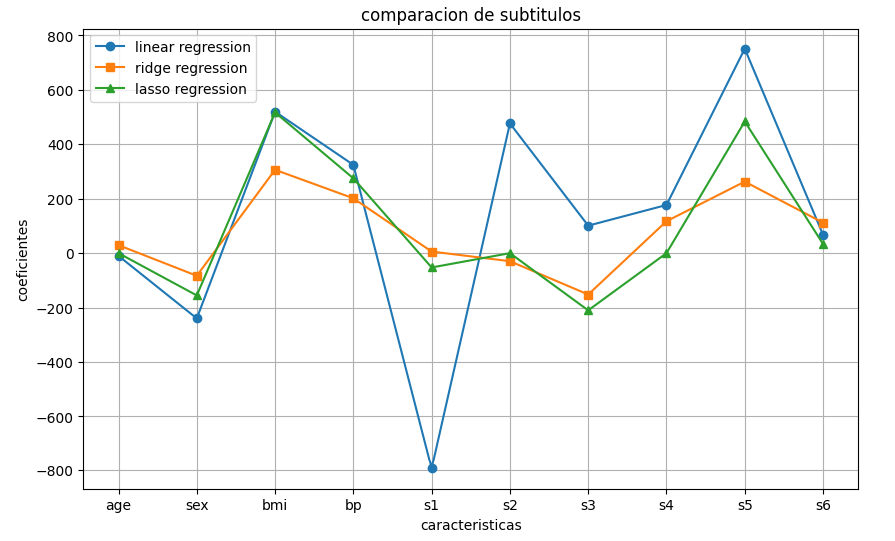
\includegraphics[width=0.9\linewidth]{imagenes/Figure1}
	\caption{Comparación entre modelos}
	\label{fig:figure1}
\end{figure}
	
	En resumen, este código carga un conjunto de datos de diabetes, define y entrena tres modelos de regresión diferentes, y luego visualiza los coeficientes de las características para cada modelo en un gráfico comparativo. Esto permite analizar cómo cada tipo de regresión (lineal, Ridge y Lasso) afecta a los coeficientes de las características, ofreciendo una comprensión visual de las diferencias entre estos métodos de regresión.
	
	\section{Conclusiones}
	Para concluir este informe, es esencial destacar los principales hallazgos y aprendizajes obtenidos a lo largo del desarrollo del proyecto de machine learning con modelos de regresión. El objetivo principal del proyecto era proporcionar una introducción práctica al uso de Python en el contexto del machine learning, permitiendo a los estudiantes experimentar con aplicaciones reales y comparar diferentes técnicas de regresión.
	
	En este proyecto, se utilizaron tres tipos de modelos de regresión: regresión lineal, regresión Ridge y regresión Lasso, aplicados al conjunto de datos de diabetes. Estos modelos fueron entrenados y evaluados, y sus coeficientes fueron visualizados para analizar cómo cada modelo maneja la regularización y afecta a los coeficientes de las características.
	
	Los resultados mostraron que la regresión Ridge y Lasso aplican regularización a los coeficientes, lo que puede ser beneficioso para manejar el sobreajuste y mejorar la generalización del modelo. La regresión Lasso, en particular, puede reducir algunos coeficientes a cero, seleccionando así un subconjunto de características, lo cual es útil para simplificar modelos y hacerlos más interpretables.
	
	Este análisis comparativo permitió a los estudiantes comprender mejor las ventajas y desventajas de cada tipo de regresión, así como la importancia de la regularización en los modelos de machine learning. Además, la implementación y visualización de estos modelos proporcionaron una experiencia práctica valiosa en el uso de bibliotecas de Python como numpy, matplotlib y sklearn.
	
	En conclusión, el proyecto no solo logró introducir a los estudiantes en el uso de Python para el machine learning, sino que también les permitió explorar y entender diferentes técnicas de regresión, fortaleciendo sus habilidades de programación y análisis de datos. Esta experiencia práctica es crucial para prepararlos para enfrentar desafíos reales en el campo de la ciencia de datos y la inteligencia artificial.
	
	\printbibliography
	
\end{document}
